%
% intro.tex
%
% (c) 2020 Prof Dr Andreas Müller, Hochschule Rapperswil
%
\bgroup

\definecolor{darkgreen}{rgb}{0,0.6,0}
\def\r{4}

\def\rad#1{
\begin{scope}[rotate=#1]
\fill[color=blue!20] (0,0) -- (-60:\r) arc (-60:60:\r) -- cycle;
\fill[color=darkgreen!20] (0,0) -- (60:\r) arc (60:180:\r) -- cycle;
\fill[color=orange!20] (0,0) -- (180:\r) arc (180:300:\r) -- cycle;

\node[color=darkgreen] at (120:3.7) [rotate={#1+30}] {Algebra};
\node[color=orange] at (240:3.7) [rotate={#1+150}] {Analysis};
\node[color=blue] at (0:3.7) [rotate={#1-90}] {Zerlegung};
\end{scope}
}

\begin{frame}
\frametitle{Intro --- Matrizen}

\vspace{-25pt}
\begin{center}
\begin{tikzpicture}[>=latex,thick]

\only<1-8>{
	\rad{-30}
	\only<2->{ \node at (90:3.0) {Rechenregeln $A^2+A+I=0$}; }
	\only<3->{ \node at (90:2.5) {Polynome $\chi_A(A)=0$, $m_A(A)=0$}; }
	\only<4->{ \node at (90:2.0) {Projektion: $P^2=P$}; }
	\only<5->{ \node at (90:1.5) {nilpotent: $N^k=0$}; }
}

\only<9-14>{
	\rad{90}
	\only<10->{ \node at (90:2.7) {Eigenbasis: $A=\sum \lambda_k P_k$}; }
	\only<11->{ \node at (90:2.2) {Invariante Räume:
		$AV\subset V, AV^\perp\subset V^\perp$}; }
}

\only<15-22>{
	\rad{210}
	\only<16->{ \node at (90:3.3) {Symmetrien}; }
	\only<17->{ \node at (90:2.8) {Skalarprodukt erhalten:
		$\operatorname{SO}(n)$}; }
	\only<18->{ \node at (90:2.3) {Konstant $\Rightarrow$ Ableitung $=0$}; }
	\only<19->{ \node at (90:1.5) {$\displaystyle \exp(A)
		= \sum_{k=0}^\infty \frac{A^k}{k!}$};
	}
}

\fill[color=red!20] (0,0) circle[radius=1.0];
\node at (0,0.25) {Matrizen};
\node at (0,-0.25) {$M_{m\times n}(\Bbbk)$};

\uncover<6->{
	\node[color=darkgreen] at (4.3,3.4) [right] {Algebra};
	\node at (4.3,2.2) [right] {\begin{minipage}{5cm}
	\begin{itemize}
	\item<6-> Algebraische Strukturen
	\item<7-> Polynome, Teilbarkeit
	\item<8-> Minimalpolynom
	\end{itemize}
	\end{minipage}};
}

\uncover<12->{
	\node[color=blue] at (4.3,0.8) [right] {Zerlegung};
	\node at (4.3,-0.4) [right] {\begin{minipage}{5cm}
	\begin{itemize}
	\item<12-> Eigenvektoren, -räume
	\item<13-> Projektionen, Drehungen
	\item<14-> Invariante Unterräume
	\end{itemize}
	\end{minipage}};
}

\uncover<20->{
	\node[color=orange] at (4.3,-1.8) [right] {Analysis};
	\node at (4.3,-3.0) [right] {\begin{minipage}{6cm}
	\begin{itemize}
	\item<20-> Symmetrien
	\item<21-> Matrix-DGL
	\item<22-> Matrix-Potenzreihen
	\end{itemize}
	\end{minipage}};
}

\end{tikzpicture}
\end{center}

\end{frame}

\egroup
